\documentclass[]{beamer}
\usepackage{beamerthemefocus}
\usepackage{amsmath}
\usepackage{bbm}
\usepackage{graphicx}
% \usepackage{xeCJK}
\usepackage{xcolor}

\setbeamertemplate{caption}[numbered]
% \setCJKmainfont{Iansui 094 Regular}
\DeclareMathOperator*{\argmax}{arg\,max}
\DeclareMathOperator*{\argmin}{arg\,min}
\newcommand{\I}[1]{\mathbbm{1}\left\{#1\right\}}
%%%%%%%%%%%%%%%%%%%%%%%%%%%%
%
%           Title and author information
%
%%%%%%%%%%%%%%%%%%%%%%%%%%%%

\title{Dynamic Bank Runs: \\ An Agent-based Approach}

\author{Toni Ricardo Eugenio dos Santos \\ [1em]
Marcio Issao Nakane \\[3em]
\small presentor: Chia Wei, Chen
}


\begin{document}
    \begin{frame}
        \maketitle
    \end{frame}

    \section{Introduction}
    \begin{frame}
    \frametitle{Bank Run in CBDC}

    Many have discussed about the possibility of run if CBDC is issues in a closed economy.
    \begin{enumerate}[<+->]
        \item Direct deposit in central bank that is fully insured
        \item Can be interest bearing as a monetary policy
        \item Competition with commercial banks, causing disintermediation by crowding out deposits \footnote{See Fernandez-Villaverde, J., D. Sanches, L. Schilling, and H. Uhlig (2021) for a model}
        \item Financial instability (Gertler and Kiyotaki, 2015)
    \end{enumerate}
    \pause
    \vfill 
    The impact could be mitigated by proper regulations and limits on the design of CBDC.

\end{frame}

\begin{frame}
    \frametitle{Bank Run Under Foreign CBDC}

    However, if CBDC is cross-border, domestic country might be out of means.

    \begin{enumerate}[<+->]
        \item Currency substitution in high-inflation country (Calvo, 1992)
        \item CBDC is digital, easy to access using mobile devices, causing faster substitution rate 
        \item Commercial banks and domestic central bank both losses deposits, causing even more severe run and financial instability.
        \item Currency substitution could ultimately impair monetary policy (Ferrari et al. 2022)
    \end{enumerate}

\end{frame}


\begin{frame}
    \frametitle{This Paper}

    Extends DD to cross-border CBDC.

    Chooses the following foreign CBDC design
    \begin{itemize}
        \item Account-base \emph{v.s. token}
        \item Retail \emph{v.s. Wholesale}
        \item Cross border
        \item Interest-bearing
    \end{itemize}
    \pause
    The domestic country has no CBDC technology, while foreign country issues cross-border CBDC that could cause capital outflows. 

\end{frame}



    \section{Model}
    \begin{frame}
    \frametitle{Consumers}

    Period 0~: \\
    Endowed with 1 unit of goods. 
    Can decide to save domestically or abroad. \\
    \vspace{2em}
    Period 1~: \\
    Consumers find out whether they are patient or not.

    \begin{equation}
        U(c_1, c_2) = \begin{cases}
            u(c_1) & \text{with prob. } \lambda \\
            u(c_2) & \text{with prob. } 1-\lambda
        \end{cases}
    \end{equation}
    If impatient, consume $c_1$ at t=1
    \\
    \vspace{2em}

    Period 2~: \\
    Patient consumers consumer $c_2$
\end{frame}

\begin{frame}
    \frametitle{Techonology}

    \begin{table}
        \begin{tabular}{cccc}
            Type & Period 0 & Period 1 & Period 2 \\
            \hline
            Short-term & 1 & 1 & \\
            
            Long-term & 1 & $l<1$ & $R>1$\\
            \hline
        \end{tabular}
    \end{table}

    Directly take the result that consumers will want to save in bank(foreign or domestic) to pool the risk.

\end{frame}

\begin{frame}
    \frametitle{Domestic Commercial Banks}

    \begin{itemize}
        \item Domestic Commercial Banks (DB) offers a demand deposit contract $(c_1, c_2)$. 
        \item DB decide to invest $y\in(0,1)$ in the short-term technology.
    \end{itemize}

    \begin{block}{Sequential Service Constraint}
        DB pays $c_1$ to depositors until all resources are exhausted.        
    \end{block}

\end{frame}

\begin{frame}[allowframebreaks]
    \frametitle{DB's problem}

    \begin{equation}
        \max_{c_1, c_2, y, {\color{red} l} \in \mathbb{R}^3_+} 
        \lambda u(c_1) + (1-\lambda)u(c_2)
    \end{equation}

    s.t. 
    \begin{subequations}
        \begin{align}
            0 &\le y \le 1 \label{eq:3a} \\
            \lambda c_1 &\le ry + (1-y)l \label{eq:3b} \\
            (1-\lambda) c_2 &\le R{\color{red} (1-l)}(1-y) + ry + (1-y)l - \lambda c_1 \label{eq:3c} \\
            c_1 &\le c_2 \label{eq:3d}
        \end{align} \label{eq:db-constraint}
    \end{subequations}
    \begin{alertblock}{Abuse of notation}
        Previously denote $l$ as liquidation price, but now denote $l$ as the proportion of long-term used for early liquidation.        
    \end{alertblock}

    \framebreak 

    Key intuitions 
    \begin{itemize}
        \item Assume bankers are Bertrand competition $\implies$ forced to maximize E.U of consumers 
        \item~\ref{eq:3b} --- might use liquidated long-term to pay $c_1$
        \item~\ref{eq:3c} --- Non-liquidated long-term plus after return is yield plus the leftover from period 1
        \item~\ref{eq:3d} --- Incentive compatibility constraint, patient consumers don't pretend to be impatient
    \end{itemize}

\end{frame}

\begin{frame}
    \frametitle{Foreign CBDC-issuing Central Bank}

    \begin{itemize}
        \item Assume perfect credible, i.e.\ no runs
        \item Justification: Fernandez-Villaverden et al. (2021) point out, certain punishment (for early withdrawal) and treatment (with patient depositors) ensures no run on CB is a DSE
        \item Foreign CBDCs are open to foreigners
        \item Constract --- $(c^*_1, c^*_2)\in \mathbb{R}^2_+$
    \end{itemize}
\end{frame}

\begin{frame}
    \frametitle{Consumers' Problem}

    Consumer invest in the highest ex-ante utility
    \begin{enumerate}
        \item Pick the contract, denote $d_i\in\{0,1\}$. $d_1=0$ means save in domestic.
        \item If utility ties, fraction $f\in[0,1]$ of consumers pick the foreign contract
    \end{enumerate}

    Consumers also decide when to withdraw their funds, denote $w_i\in \{1,2\}$. Note that $w_i=w_i (w_{-i})$
    \vfill
    Capital account constraint --- Total investment in foreign asset must not exceed $k$
    \begin{itemize}
        \item Exogenous ceiling
        \item Regulation restriction
    \end{itemize}
\end{frame}

    \section{Simulation}
    \begin{frame}
    \frametitle{Parameters}

    \begin{enumerate}
        \item ``r''s --- $r, r_1, r_2, R$
        \item Impatient threshold $\tau$
    \end{enumerate}

    \vfill 
    \pause
    The authors set 
    \begin{itemize}
        \item $r = 0.8$
        \item $r_1 \in \{1.001, 1.003, 1.005, 1.007, 1.009\}$
        \item $r_2 = 1.03$
        \item $R = 1.05$
        \item $\tau \in \{0.4, 0.6, 0.8\}$
    \end{itemize}
    \vfill
    Each combination of parameter is simulated 100 times, each with 1,000 cycles(3 subperiod of Diamond Dybvig environment each)
    
\end{frame}

\begin{frame}[plain]
    \setcounter{figure}{2}
    \begin{figure}
        \centering
        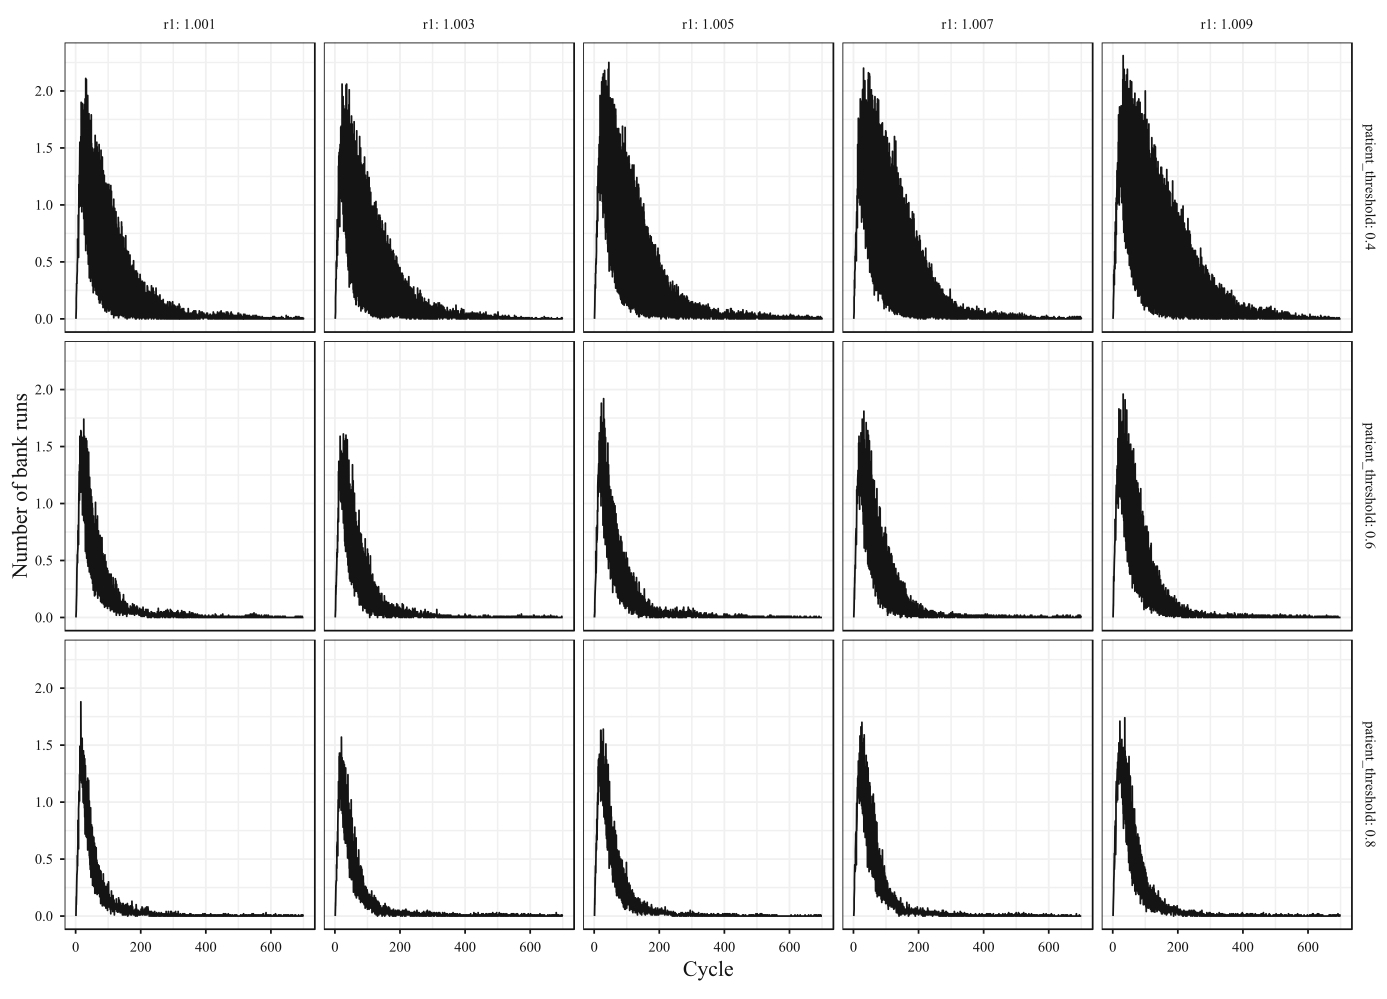
\includegraphics[width=\textwidth]{fig/fig3.jpeg}
        \caption{Average number of bank runs}
        \label{fig:num_run}
    \end{figure}
\end{frame}

\begin{frame}[plain]
    \begin{figure}
        \centering
        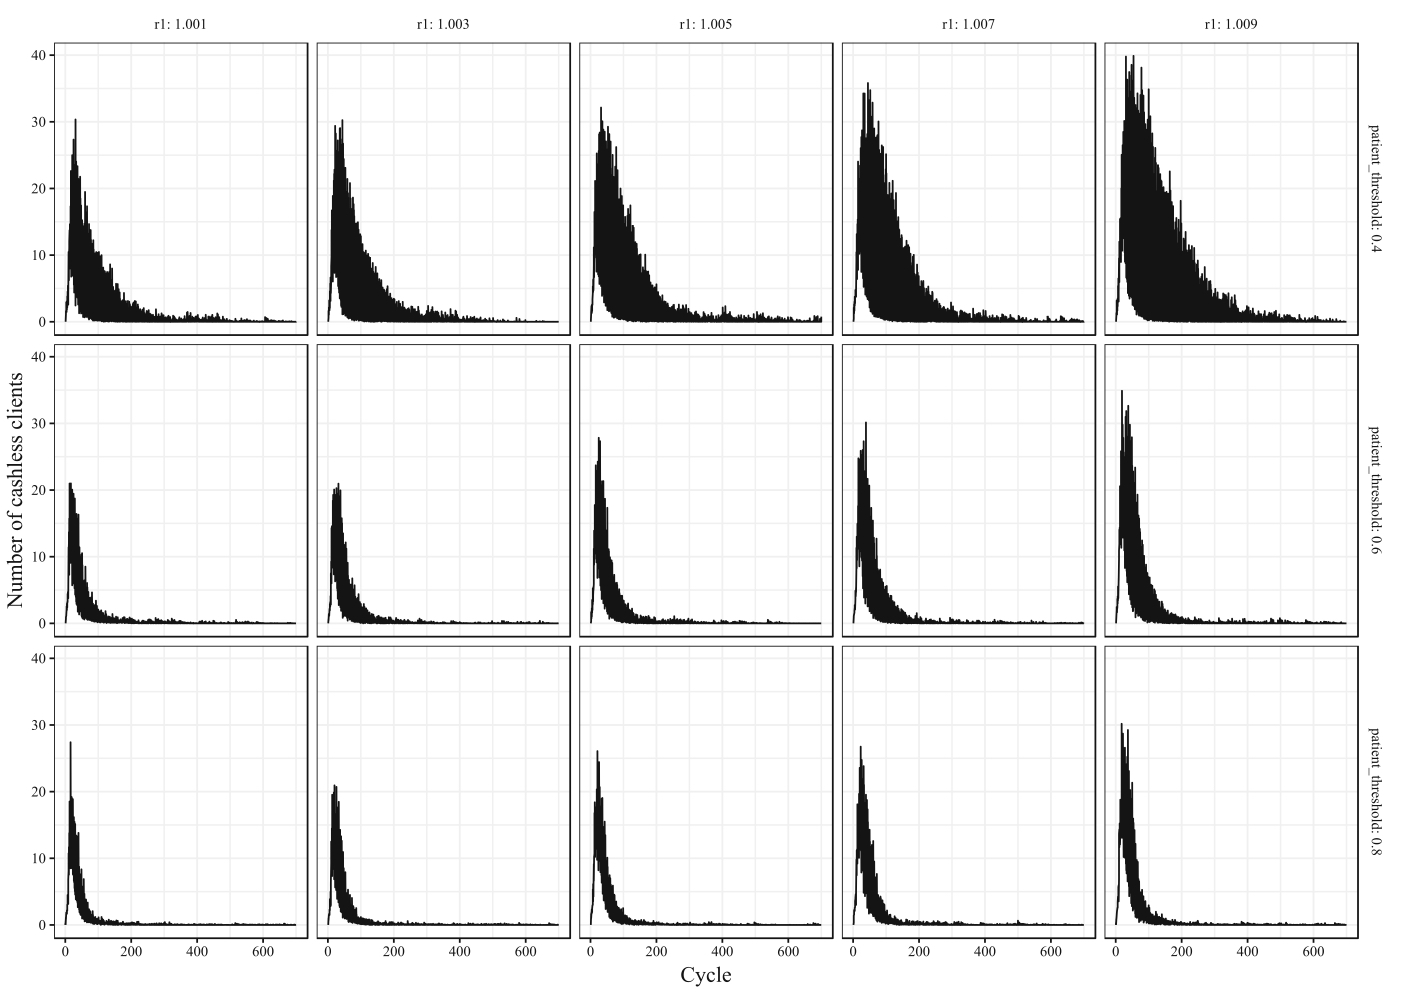
\includegraphics[width=\textwidth]{fig/fig4.jpeg}
        \caption{Average number of clients failed to withdraw}
        \label{fig:num_run}
    \end{figure}
\end{frame}

\begin{frame}[plain]
    \begin{figure}
        \centering
        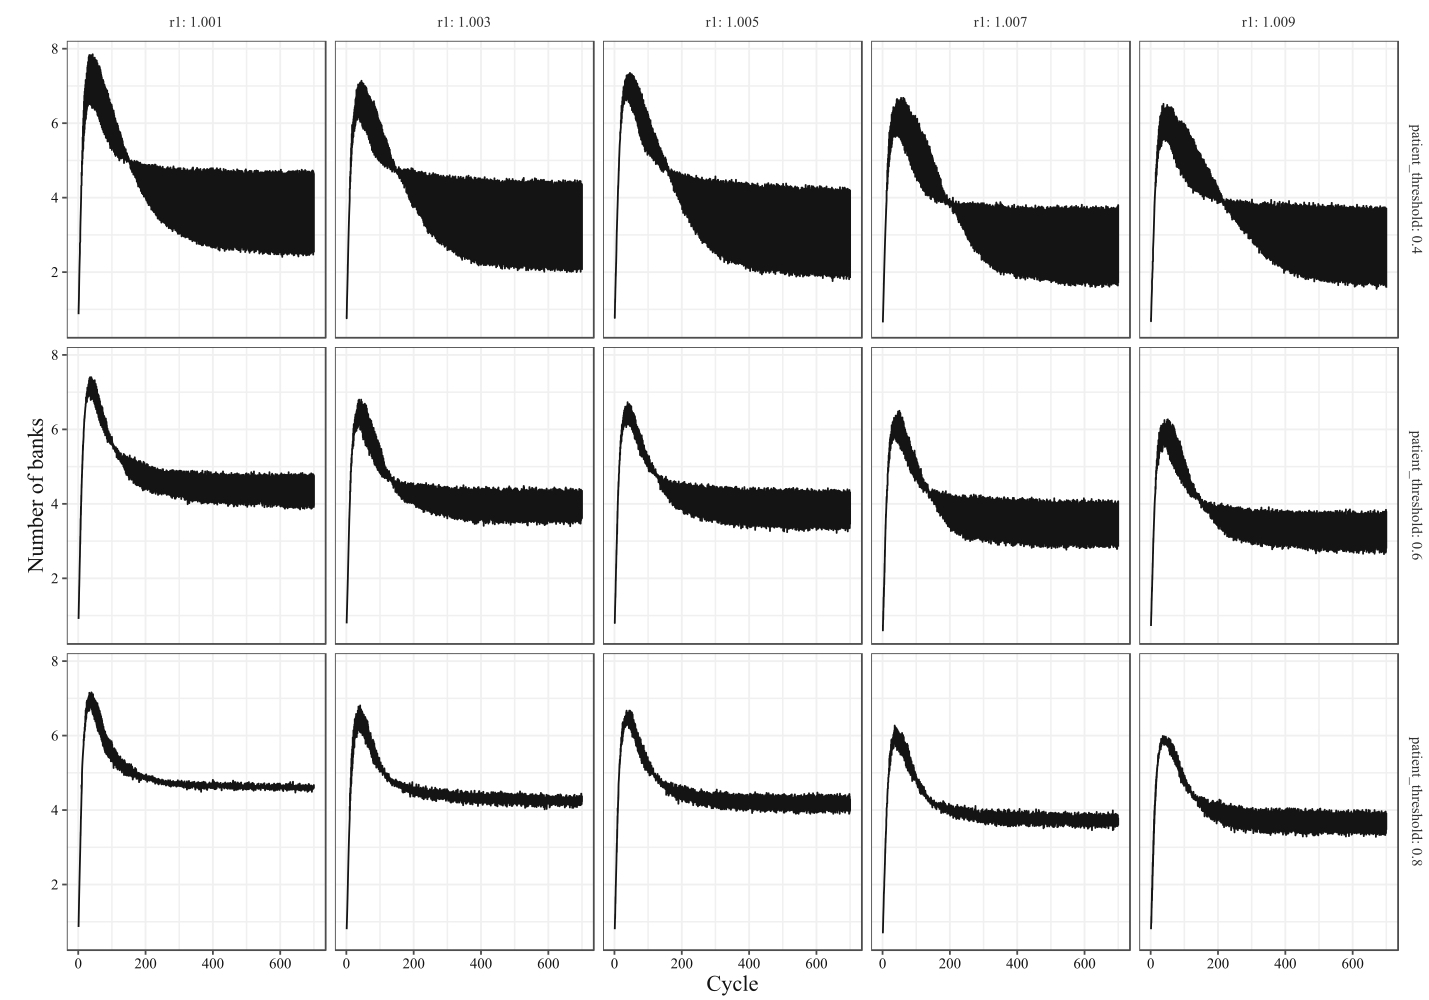
\includegraphics[width=\textwidth]{fig/fig5.jpeg}
        \caption{Average number of banks}
        \label{fig:num_run}
    \end{figure}
\end{frame}

\setcounter{figure}{6}

\begin{frame}[plain]
    \begin{figure}
        \centering
        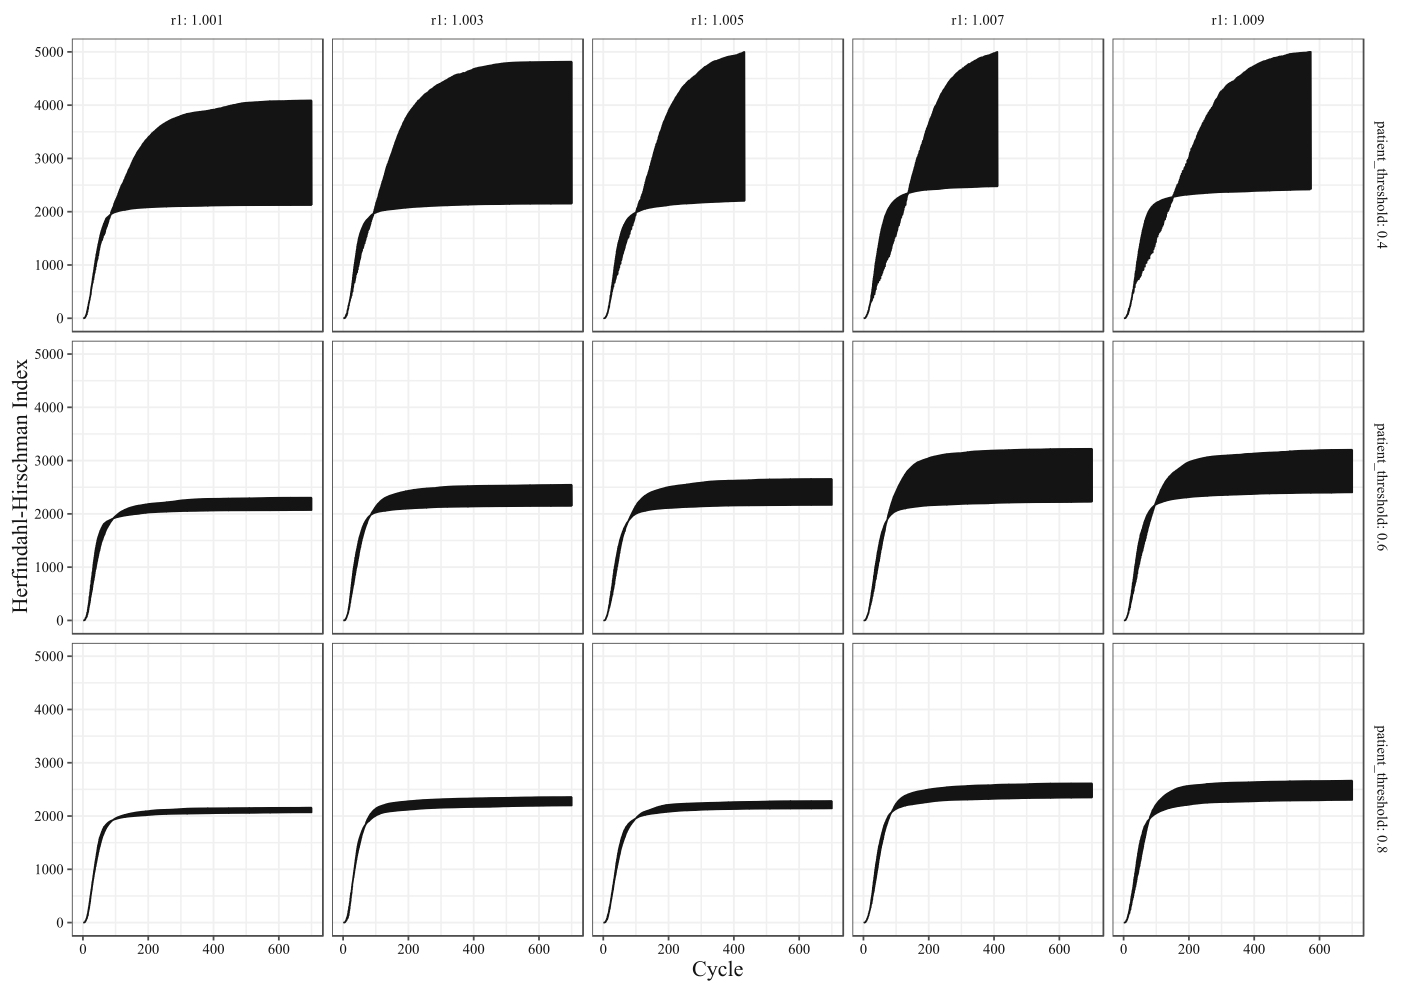
\includegraphics[width=\textwidth]{fig/fig7.jpeg}
        \caption{Average Herfindahl-Hirschman index (Sum of market share squared)}
        \label{fig:num_run}
    \end{figure}
\end{frame}


\begin{frame}[plain]
    \begin{figure}
        \centering
        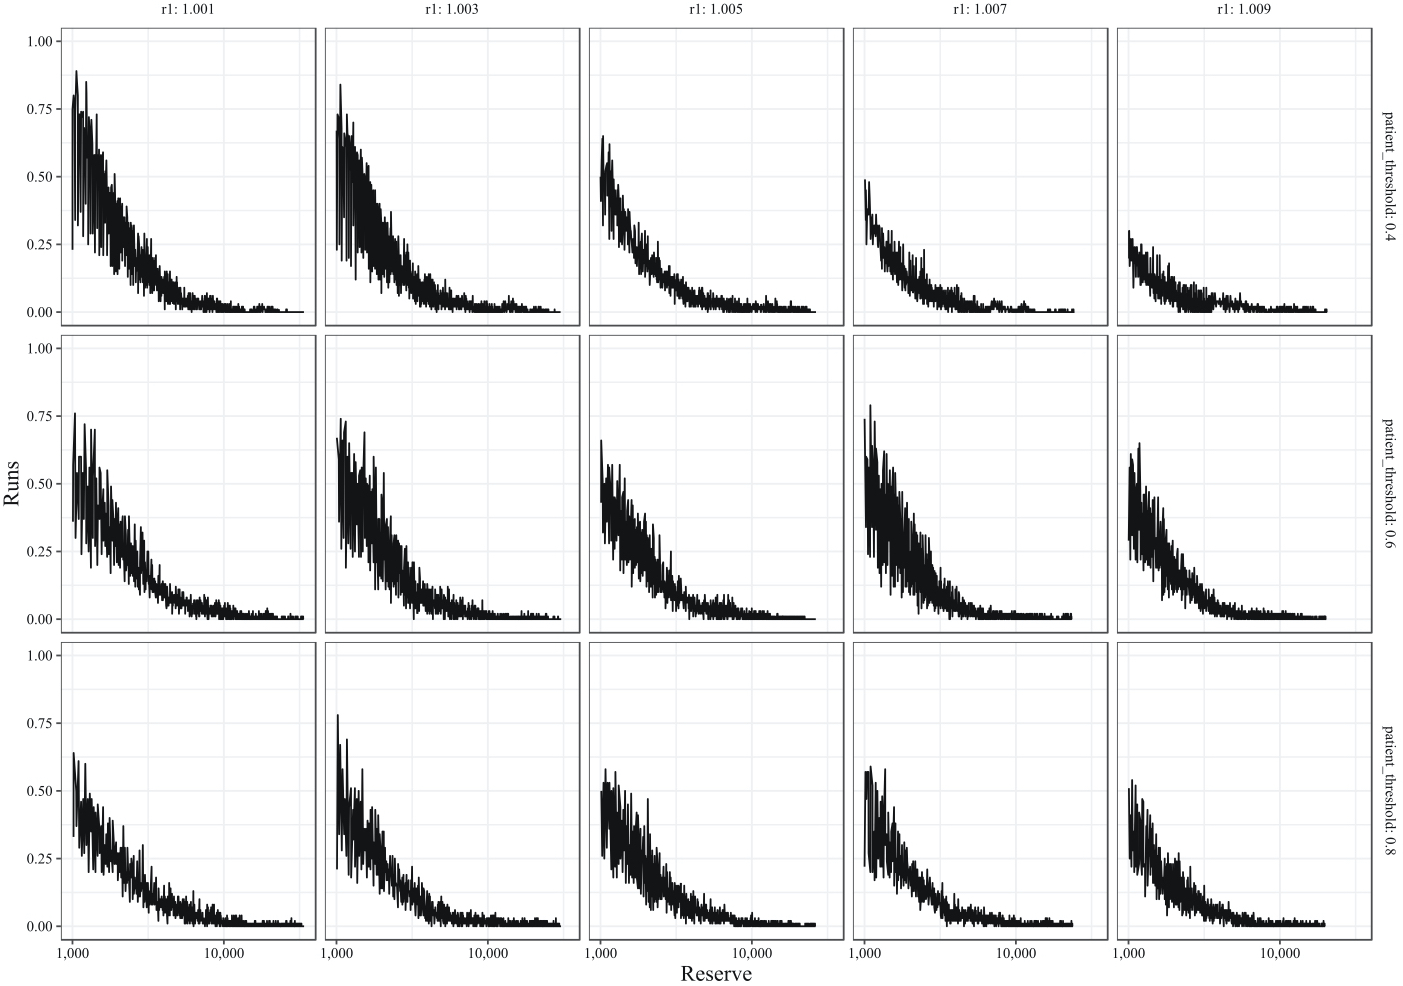
\includegraphics[width=\textwidth]{fig/fig8.jpeg}
        \caption{Bank reserve versus number of runs}
        \label{fig:num_run}
    \end{figure}
\end{frame}
    
    \section{Extension}
    \begin{frame}
    \frametitle{Allowing Wealth Accumulation}

    In previous baseline model, each agent returns to the unit endowment.
    \pause
    \vfill 
    If we allow depositors to accumulate wealth: 
    \begin{enumerate}
        \item Bank reserve large, harder for bank run to occur.
        \item Withdrawal amount increases, easier for bank run to occur.
    \end{enumerate}

    The extension checks if this scenario is possible.

\end{frame}

\begin{frame}
    \frametitle{Modification --- Wealth}

    Some agents might never withdraw in t=1
    \begin{itemize}
        \item Wealth follows a geometric progression growth 
    \end{itemize}
    \vfill 
    \begin{itemize}
        \item $\omega_i$ --- available wealth 
        \item 1 unit of endowment at each t=0 
        \item Agents allocate $\omega_i$ in asset market or deposit
        \item \color{red}{Spends $\omega_i$ each cycle --- (Sort of) Hand to mouth setting}
    \end{itemize}
\end{frame}

\begin{frame}
    \frametitle{Allocation decision of $\omega_i$}

    Agents not clients of bank 
    \begin{itemize}
        \item Impatient --- Spent all in t=1. $\omega_{i, t+1}=0$
        \item Patient --- No spending in t=1, receive $R\omega_i$ in t=2, spend $\omega_i$
    \end{itemize}

    Agents who are clients of bank
    \begin{itemize}
        \item Impatient --- received $r_1 \omega_i$ in t=1, spend $\omega_i$ in t=1
        \item Patient --- No spending in t=1, receive $r_2 \omega_i$ in t=2, spend $\omega_i$
    \end{itemize}
\end{frame}

\begin{frame}
    \frametitle{Banks' allocation}

    \emph{The authors did not mentioned the modification on the formation and allocation of banks.}

    The orders of offering money is the same 
    \begin{enumerate}
        \item Liquid assests
        \item Reserves 
        \item Illiquid assets
    \end{enumerate}

    If the bank has not enough to pay, some clients receive nothing, and the bank fails.
\end{frame}

\begin{frame}
    \frametitle{Thoughts}

    \begin{itemize}[<+->]
        \item A great start to explore dynamic bank runs.
        \item Bank run emerges from simple imitation rule, which considers only limited knowledge from the environment(neighbors), not a global information.
        \item Endogenously selection of becoming clients of bank.
    \end{itemize}
\end{frame}

\begin{frame}
    \frametitle{Improvements and criticisms}
    \pause
    Criticisms
    \begin{enumerate}[<+->]

        \item Consumption smoothing
        \item Expected value of a forecast not described clearly
    \end{enumerate}
    \vfill
    Adjustment and Improvements
    \begin{enumerate}
        \item Existing large banks. Endogenous bank formation is not necessary in most applications. 
        \item Exogenous bank-depositor network --- Spacial network is not enough.
        \item Consumption and preference shock should be endogenous and follow a transition process.
    \end{enumerate}

\end{frame}
\end{document}